\begin{center}
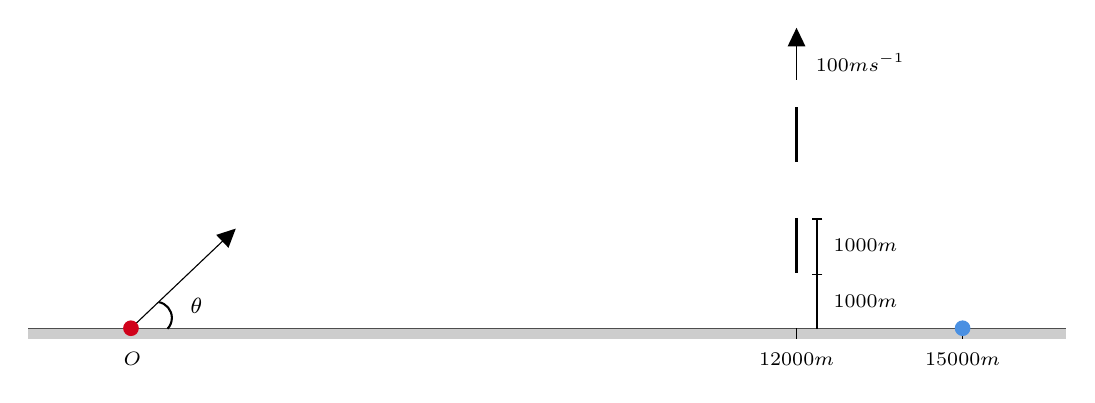
\begin{tikzpicture}[x=0.75pt,y=0.75pt,yscale=-1,xscale=1]

%Straight Lines [id:da45198010726670845] 
\draw    (80.33,155) -- (580.33,155) ;
%Shape: Rectangle [id:dp9890398319964502] 
\draw  [draw opacity=0][fill={rgb, 255:red, 155; green, 155; blue, 155 }  ,fill opacity=0.5 ] (80.33,155) -- (580.33,155) -- (580.33,160.33) -- (80.33,160.33) -- cycle ;
%Straight Lines [id:da9896789843028051] 
\draw    (129.83,155) -- (178.16,109.07) ;
\draw [shift={(180.33,107)}, rotate = 496.45] [fill={rgb, 255:red, 0; green, 0; blue, 0 }  ][line width=0.08]  [draw opacity=0] (8.93,-4.29) -- (0,0) -- (8.93,4.29) -- cycle    ;
%Shape: Arc [id:dp2518682859253052] 
\draw  [draw opacity=0][line width=0.75]  (143.2,142.42) .. controls (146.79,143.06) and (149.52,146.19) .. (149.54,149.96) .. controls (149.55,152.02) and (148.76,153.88) .. (147.45,155.27) -- (141.84,150) -- cycle ; \draw  [line width=0.75]  (143.2,142.42) .. controls (146.79,143.06) and (149.52,146.19) .. (149.54,149.96) .. controls (149.55,152.02) and (148.76,153.88) .. (147.45,155.27) ;
%Shape: Circle [id:dp13299007709992905] 
\draw  [color={rgb, 255:red, 208; green, 2; blue, 27 }  ,draw opacity=1 ][fill={rgb, 255:red, 208; green, 2; blue, 27 }  ,fill opacity=1 ] (126.33,155) .. controls (126.33,153.07) and (127.9,151.5) .. (129.83,151.5) .. controls (131.77,151.5) and (133.33,153.07) .. (133.33,155) .. controls (133.33,156.93) and (131.77,158.5) .. (129.83,158.5) .. controls (127.9,158.5) and (126.33,156.93) .. (126.33,155) -- cycle ;
%Straight Lines [id:da7363174446974949] 
\draw    (450.5,155.13) -- (450.5,160.13) ;
%Straight Lines [id:da8507054156705689] 
\draw    (530.5,155.13) -- (530.5,160.13) ;
%Shape: Circle [id:dp0875287559905249] 
\draw  [color={rgb, 255:red, 74; green, 144; blue, 226 }  ,draw opacity=1 ][fill={rgb, 255:red, 74; green, 144; blue, 226 }  ,fill opacity=1 ] (527,155) .. controls (527,153.07) and (528.57,151.5) .. (530.5,151.5) .. controls (532.43,151.5) and (534,153.07) .. (534,155) .. controls (534,156.93) and (532.43,158.5) .. (530.5,158.5) .. controls (528.57,158.5) and (527,156.93) .. (527,155) -- cycle ;
%Straight Lines [id:da9565901506094769] 
\draw [line width=1.25]    (450.5,101.79) -- (450.5,128.46) ;
%Straight Lines [id:da8590807071227391] 
\draw [line width=1.25]    (450.5,48.46) -- (450.5,75.12) ;
%Straight Lines [id:da1250805630667582] 
\draw [line width=0.5]    (460.36,102.39) -- (460.36,129.06) ;
%Straight Lines [id:da2542517178085071] 
\draw [line width=0.5]    (462.94,102.39) -- (457.77,102.39) ;
%Straight Lines [id:da9006595888470921] 
\draw [line width=0.5]    (462.94,129.06) -- (457.77,129.06) ;

%Straight Lines [id:da4594515235335257] 
\draw [line width=0.5]    (460.36,129.06) -- (460.36,155.3) ;
%Straight Lines [id:da8735781741018898] 
\draw [line width=0.5]    (450.5,13.25) -- (450.5,35.46) ;
\draw [shift={(450.5,10.25)}, rotate = 90] [fill={rgb, 255:red, 0; green, 0; blue, 0 }  ][line width=0.08]  [draw opacity=0] (8.93,-4.29) -- (0,0) -- (8.93,4.29) -- cycle    ;

\draw (161.33,144) node  [font=\footnotesize]  {$\theta$};
\draw (450.5,170) node  [font=\scriptsize]  {$12000m$};
\draw (530.5,170) node  [font=\scriptsize]  {$15000m$};
\draw (483.7,115.2) node  [font=\scriptsize]  {$1000m$};
\draw (483.7,142.18) node  [font=\scriptsize]  {$1000m$};
\draw (481.2,26.85) node  [font=\scriptsize]  {$100ms^{-1}$};
\draw (130.5,170) node  [font=\scriptsize]  {$O$};

\end{tikzpicture}
\end{center}
